\let\negmedspace\undefined
\let\negthickspace\undefined
\documentclass[journal]{IEEEtran}
\usepackage[a5paper, margin=10mm, onecolumn]{geometry}
\usepackage{lmodern} % Ensure lmodern is loaded for pdflatex
\usepackage{tfrupee} % Include tfrupee package

\setlength{\headheight}{1cm} % Set the height of the header box
\setlength{\headsep}{0mm}     % Set the distance between the header box and the top of the text
\usepackage{float}
\usepackage{gvv-book}
\usepackage{gvv}
\usepackage{cite}
\usepackage{amsmath,amssymb,amsfonts,amsthm}
\usepackage{algorithmic}
\usepackage{graphicx}
\usepackage{textcomp}
\usepackage{xcolor}
\usepackage{txfonts}
\usepackage{listings}
\usepackage{enumitem}
\usepackage{mathtools}
\usepackage{gensymb}
\usepackage{comment}
\usepackage[breaklinks=true]{hyperref}
\usepackage{tkz-euclide} 
\usepackage{listings}
\usepackage{gvv}                                        
\def\inputGnumericTable{}                                 
\usepackage[latin1]{inputenc}                                
\usepackage{color}                                            
\usepackage{array}                                            
\usepackage{longtable}                                       
\usepackage{calc}                                             
\usepackage{multirow}                                         
\usepackage{hhline}                                           
\usepackage{ifthen}                                           
\usepackage{lscape}
\usepackage{listings}
\begin{document}

\bibliographystyle{IEEEtran}
\vspace{3cm}
	
\title{XE 2008 18-34}
\author{EE24BTECH11005 - Arjun Pavanje}
% \maketitle
% \newpage
% \bigskip

{\let\newpage\relax\maketitle}
\begin{enumerate}
\setcounter{enumi}{39}
	\item In finding a root of the equation: $x^2-6x+5=0$ the Newton-Ralphson method achieves an order of convergance equal to,
		\begin{enumerate}
				\begin{multicols}{2}
				\item $1.0$
						\columnbreak
					\item $1.67$
				\end{multicols}
				\begin{multicols}{2}
					\item $2.0$
				\columnbreak
			\item $2.5$
				\end{multicols}
		\end{enumerate}
	\item Consider a $1-D$ adiabatic, inviscid, compressible Now of air $\brak{R = 287 J/Kg-K, c_r = 718 J/Kg-K}$ through a duct of constant cross-sectional area $A=1 m$. If the volumetric flow rate is $Q=680 m^3/s$ and stagnation temperature is $T, = 580.05 K$, then the air temperature inside the duct is
				\begin{enumerate}
				\begin{multicols}{2}
			\item $300K$
				\columnbreak
			\item $350K$
				\end{multicols}
				\begin{multicols}{2}
				\item $400K$
					\columnbreak
				\item $450K$ 
				\end{multicols}
		\end{enumerate}
	\item A two stage chemical rocket, having the same specific impulse $\brak{l_{sp}}$ of $300 s$ for both the stages is designed in such a way that the payload ratio and the structural ratio are same for both the stages. The second stage of the rocket has following mass distribution:\\
		Propellant Mass = $10208 kg$\\
		Structural Mass = $1134 kg$\\
		Payload Mass = $1700 kg$
		$g_e = 9.8 m/s2$\\
		If the rocket is fired from rest and it flies in a zero gravity field and a drag free environment, the final velocity attained by the payload is
	\begin{enumerate}
	\begin{multicols}{2}
		\item  $9729.3m/s$
		 \columnbreak
		\item  $897.3m/s$
    \end{multicols}
    \begin{multicols}{2}
	\item $9360.2m/s$ 
    \columnbreak
\item $8973.2m/s$
    \end{multicols}
\end{enumerate}
\item A missile with a Ramjet engine is flying in air. The temperature at the inlet and the outlet of the combustor are $1200 K$ and $2500 K$ respectively. The heating value of the fuel is $43 MJ/kg$ and the burner efficiency is $90\%$. Considering the working fluid to be air $\brak{C_p = 1005 J/kgK, \gamma = 1.4}$, The for this engine is equal to: $\frac{\text{fuel}}{\text{air}}$ ratio $\brak{f=\frac{m_f}{m_a}}$
	\begin{enumerate}
    \begin{multicols}{2}
        \item $0.032$
    \columnbreak
        \item $0.036$
    \end{multicols}
    \begin{multicols}{2}
        \item $0.042$
    \columnbreak
        \item $0.026$
    \end{multicols}
\end{enumerate}
\item The trim curves of an aircraft are of the form $C_m \brak{0.05-0.2\delta_r}-0.1C_l$, where the elevator deflection angle, $\delta_e$, is in radians. The change in elevator deflection needed to increase the lift coefficient from $0.4$ to $0.9$ is:
	\begin{enumerate}
    \begin{multicols}{2}
	\item $-0.5$ radians
    \columnbreak
\item $-0.25$ radians
    \end{multicols}
    \begin{multicols}{2}
	\item $0.25$ radians
    \columnbreak
\item $0.5$ radians
    \end{multicols}
\end{enumerate}
\item If $e$ is the base of the natural logarithms then the equation of the tangent from the origin to the curve $y=e^x$ is
	\begin{enumerate}
    \begin{multicols}{2}
        \item $y=x$
    \columnbreak
        \item $y=\pi x$
    \end{multicols}
    \begin{multicols}{2}
	\item $y=\frac{x}{e}$
    \columnbreak
        \item $y=ex$
    \end{multicols}
\end{enumerate}
\item Consider a potential flow over a finite wing with the following circulation distribution
\begin{figure}[H]
			\centering
			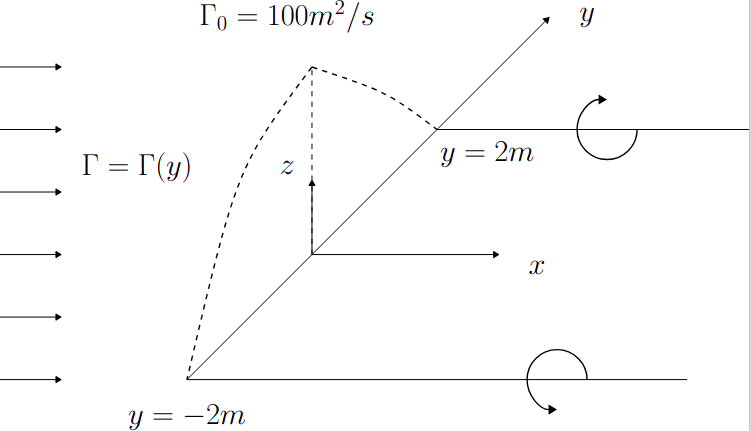
\includegraphics[scale=0.4]{figs/q46.png}
			\label{stemplot}
		\end{figure}
\begin{align*}
	\Gamma\brak{y}=100\sqrt{1-\brak{\frac{2y}{4}}^2} m^2/s
\end{align*}
	\begin{enumerate}
    \begin{multicols}{2}
        \item $0.125$ radians
    \columnbreak
        \item $-0.125$ radians
    \end{multicols}
    \begin{multicols}{2}
	\item $0.125\sqrt{1=\brak{\frac{y}{2}}^2}$ radians
    \columnbreak
        \item $-0.125\sqrt{1=\brak{\frac{y}{2}}^2}$ radians

    \end{multicols}
\end{enumerate}
\item The inlet stagnation temperature for a single stage axial compressor is $300 K$ and the stage efficiency is $0.80$. Following conditions exist at the mean radius of the rotor blade: \\
	Blade speed $= 200 m/s$\\
	Axial flow velocity $=160 m/s$\\
	Intet blade angle $\beta_1 = 44\degree$\\
	Outlet blade angle $\beta_2 = 14\degree$\\
	$C_p 1005 J/kgK \text{and} y= 1.4$\\
	What is the stagnation pressure ratio $\brak{\text{PRS}}$ for this compressor?

	\begin{enumerate}
    \begin{multicols}{2}
        \item $1.41$
    \columnbreak
        \item $1.37$
    \end{multicols}
    \begin{multicols}{2}
        \item $1.51$
    \columnbreak
        \item $1.23$
    \end{multicols}
\end{enumerate}
\textbf{Common Data for Questions 48 and 49:}\\
Consider a simply supported beam of length $L$, carrying a bracket welded at its center. The bracket carries a vertical load, $P$, as shown in the figure. Dimensions of bracket are $a=0.1L$. The beam has a square cross-section of dimension $h \times h$.
\item Bending moment diagram is given by,
\begin{figure}[H]
			\centering
			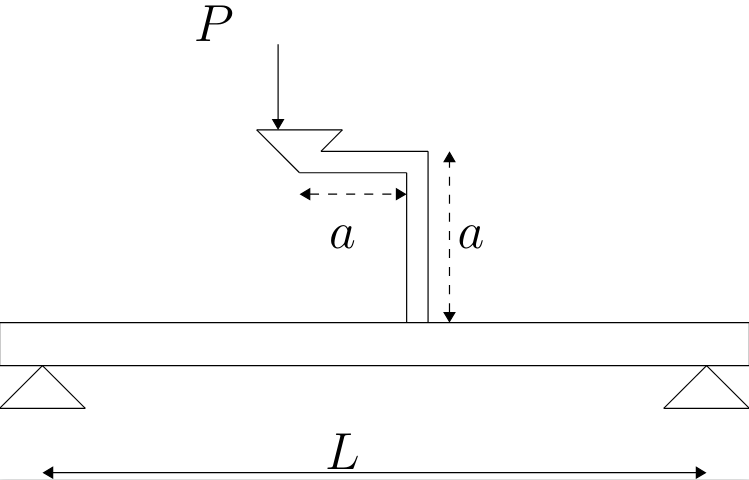
\includegraphics[scale=0.4]{figs/para.png}
			\label{stemplot}
		\end{figure}

	\begin{enumerate}

			\begin{multicols}{2}
		\item . \begin{figure}[H]
			\centering
			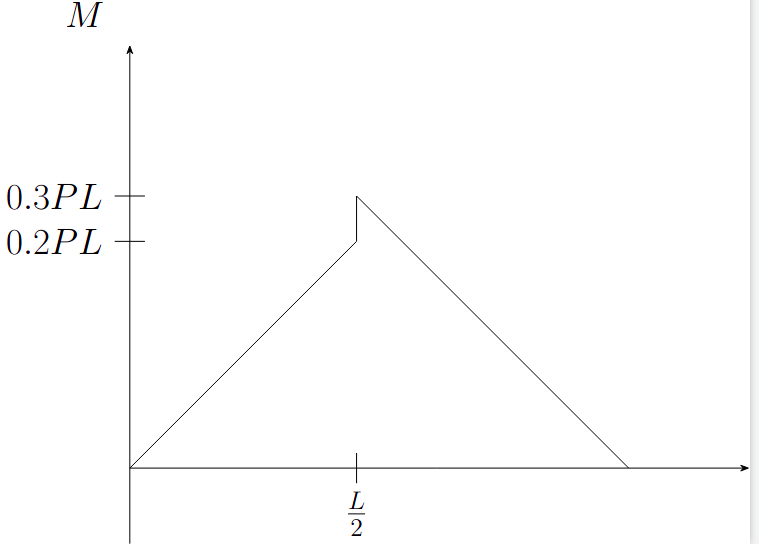
\includegraphics[scale=0.2]{figs/a.png}
			\label{stemplot}
		\end{figure}
				\columnbreak
			\item . \begin{figure}[H]
			\centering
			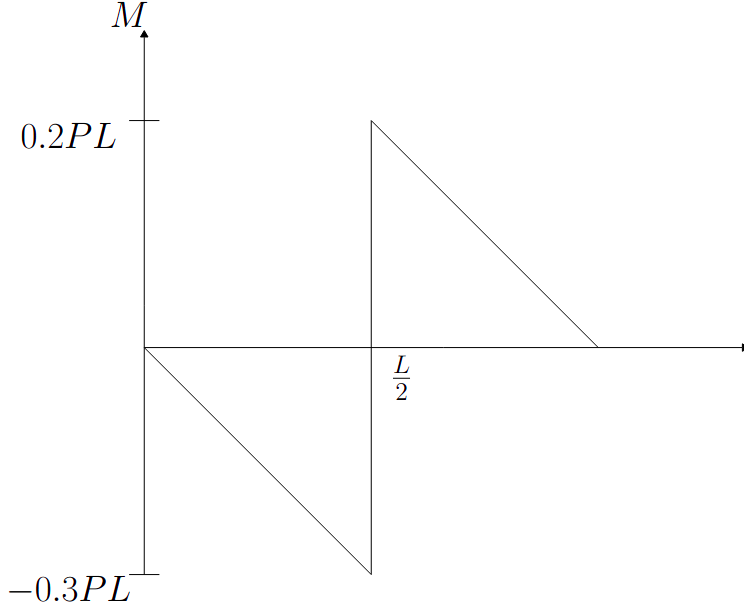
\includegraphics[scale=0.2]{figs/b.png}
			\label{stemplot}
		\end{figure}
			\end{multicols}
			\begin{multicols}{2}
			\item . \begin{figure}[H]
			\centering
			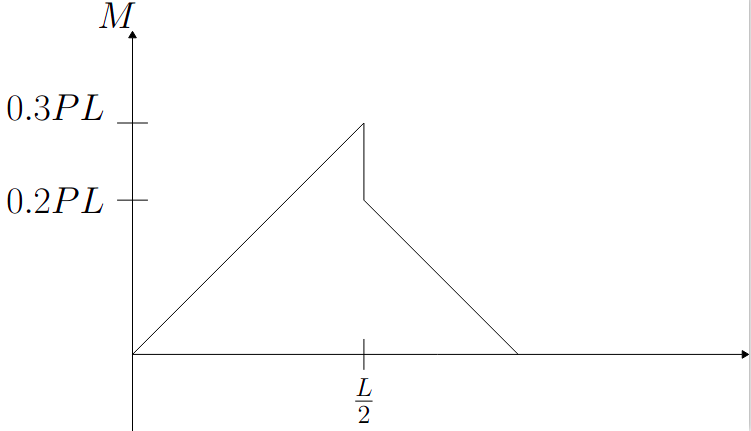
\includegraphics[scale=0.2]{figs/c.png}
			\label{stemplot}
		\end{figure}
				\columnbreak
			\item . \begin{figure}[H]
			\centering
			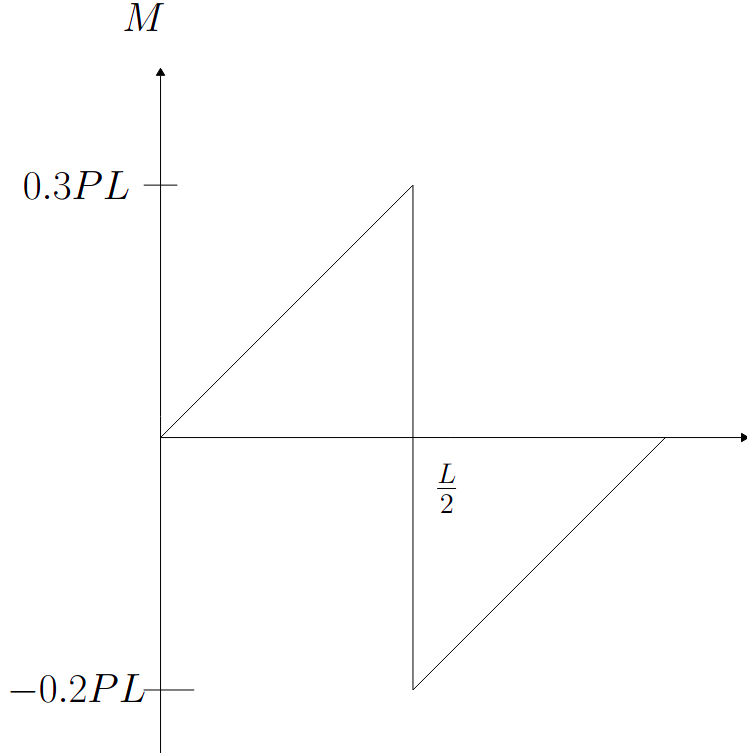
\includegraphics[scale=0.2]{figs/d.png}
			\label{stemplot}
		\end{figure}
			\end{multicols}
		\end{enumerate}
\item Maximum value of shear stress is,
	\begin{enumerate}
    \begin{multicols}{2}
        \item $0.67P/h^2$
    \columnbreak
\item $1.33P/h^2$
    \end{multicols}
    \begin{multicols}{2}
        \item $1.5P/h^2$
    \columnbreak
\item $0.9 P/h^2$
    \end{multicols}
\end{enumerate}
\textbf{Statement for Linked Answer Questions 50 and 51:}\\
Consider a potential flow over a spinning cylinder. The stream function is given as,
\begin{align*}
	\psi =\brak{V_{\infty}r\sin\theta}\brak{1=\frac{R^2}{r^2}}+\frac{\Gamma}{2\pi}\ln\frac{r}{R}
\end{align*}
where \\
Free stream velocity, $V_{\infty}=25m/s$\\
Cylinder radius, $R=1m$\\
Circulation, $\Gamma =50\pi m^2/s$
\begin{figure}[H]
			\centering
			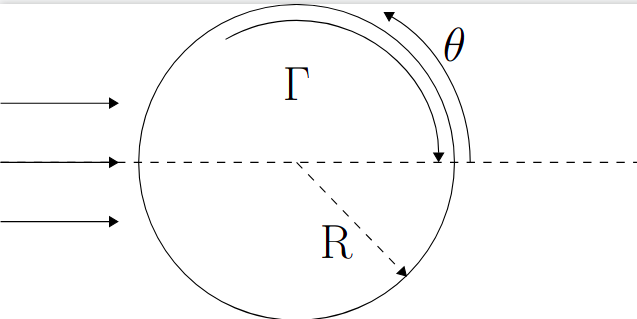
\includegraphics[scale=0.4]{figs/q50.png}
			\label{stemplot}
		\end{figure}
\item The radial and azimuthal velocities on the cylinder surface at $\theta=\frac{\pi}{2}$ are,
	\begin{enumerate}
    \begin{multicols}{2}
        \item $V_r=0m/s, V_0=-75m/s$
        \columnbreak
        \item $V_r=0m/s, V_0=75m/s$
    \end{multicols}
    \begin{multicols}{2}
        \item $V_r=0m/s, V_0=-25m/s$
        \columnbreak
        \item $V_r=0m/s, V_0=25m/s$
    \end{multicols}
\end{enumerate}
\item The stagnantation points are located at
\begin{enumerate}
    \begin{multicols}{2}
        \item $210\degree$ and $330\degree$
        \columnbreak
        \item $240\degree$ and $300\degree$
    \end{multicols}
    \begin{multicols}{2}
        \item $30\degree$ and $150\degree$
        \columnbreak
        \item $60\degree$ and $120\degree$
    \end{multicols}
\end{enumerate}
\textbf{Statement for Linked Answer Questions 52 and 53:}\\
 An aircraft with an IDEAL Turbojet engine is flying at $200 m/s$ at an altitude where the ambient pressure is equal to $0.8 bar$. The stagnation pressure and temperature at the inlet of the turbine are $6 bar$ and $1400 K$ respectively. The change in specific enthalpy across the compressor is $335 kJ/kg$. Assume the fuel flow rate to be very small in comparison to the air flow rate and consider $C_p = 1117 J/kgK$ and $\gamma = 1.3$.
\item What is the stagnantation pressure at the inlet of the nozzle,
\begin{enumerate}
    \begin{multicols}{2}
        \item $2.8 bar$
        \columnbreak
        \item $5.7 bar$
    \end{multicols}
    \begin{multicols}{2}
        \item $2.1 bar$
        \columnbreak
        \item $6.3 bar$
    \end{multicols}
\end{enumerate}

\end{enumerate}

\end{document}
